\documentclass{article}
\usepackage[margin=0.75in]{geometry}
\usepackage{tikz}
\usetikzlibrary{positioning,arrows.meta,calc,shapes.geometric}
\usepackage{tcolorbox}
\usepackage{xcolor}
\usepackage{skak}

\newcommand{\benchmark}{ChessChain}

\begin{document}

\begin{figure}[t]
    \centering

    % Chess problem - Version 3: Board + Flow diagram side by side
    \begin{tcolorbox}[
        title=\textbf{Chess: Minimax Search} \hfill {\small\colorbox{orange!20}{Easy} \quad 6 orderings},
        colframe=orange!70!black,
        colback=orange!3,
        boxrule=0.8pt,
        width=\textwidth
    ]
    \small

    \begin{minipage}{0.32\textwidth}
        \centering
        \textbf{Board State}
        \vspace{0.2cm}

        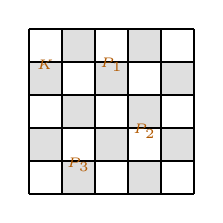
\begin{tikzpicture}[scale=0.42]
            % Draw 5x5 board
            \foreach \x in {0,...,4} {
                \foreach \y in {0,...,4} {
                    \pgfmathparse{mod(\x+\y,2) ? "gray!25" : "white"}
                    \fill[\pgfmathresult] (\x,\y) rectangle (\x+1,\y+1);
                }
            }
            \draw[thick] (0,0) grid (5,5);
            % Knight at (0,4)
            \node at (0.5,4.5) {\small$\symknight$};
            % Pawns with labels
            \node at (2.5,4.5) {\small$\sympawn$};
            \node[font=\tiny, orange!70!black] at (2.5,3.9) {$P_1$};
            \node at (3.5,2.5) {\small$\sympawn$};
            \node[font=\tiny, orange!70!black] at (3.5,1.9) {$P_2$};
            \node at (1.5,1.5) {\small$\sympawn$};
            \node[font=\tiny, orange!70!black] at (1.5,0.9) {$P_3$};
            % Knight label
            \node[font=\tiny, orange!70!black] at (0.5,3.9) {$K$};
        \end{tikzpicture}

        \vspace{0.2cm}
        {\scriptsize Knight captures all pawns}
    \end{minipage}%
    \hfill%
    \begin{minipage}{0.65\textwidth}
        \centering
        \textbf{Dependency Graph}
        \vspace{0.1cm}

        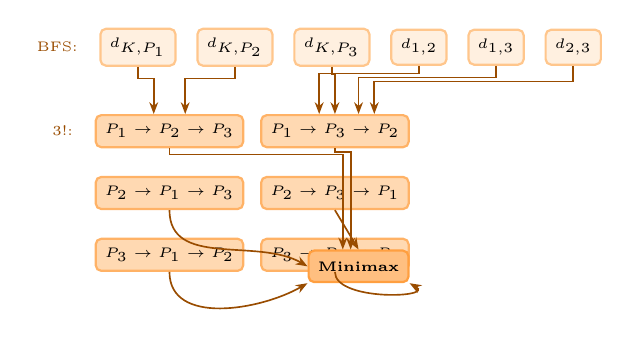
\begin{tikzpicture}[
            node distance=0.4cm and 0.5cm,
            every node/.style={font=\tiny},
            bfs/.style={draw, rounded corners=2pt, fill=orange!12, minimum width=0.7cm, minimum height=0.4cm, thick, draw=orange!45},
            gamenode/.style={draw, rounded corners=2pt, fill=orange!30, minimum width=1.6cm, minimum height=0.4cm, thick, draw=orange!60},
            outputnode/.style={draw, rounded corners=2pt, fill=orange!50, minimum width=0.9cm, minimum height=0.4cm, thick, draw=orange!75, font=\tiny\bfseries},
            arrow/.style={-{Stealth[length=1.5mm]}, semithick, orange!60!black}
        ]
            % BFS layer - distances
            \node[bfs] (d1) {$d_{K,P_1}$};
            \node[bfs, right=0.25cm of d1] (d2) {$d_{K,P_2}$};
            \node[bfs, right=0.25cm of d2] (d3) {$d_{K,P_3}$};
            \node[bfs, right=0.25cm of d3] (d4) {$d_{1,2}$};
            \node[bfs, right=0.25cm of d4] (d5) {$d_{1,3}$};
            \node[bfs, right=0.25cm of d5] (d6) {$d_{2,3}$};

            % Label
            \node[font=\tiny, orange!60!black, anchor=east] at ([xshift=-0.15cm]d1.west) {BFS:};

            % Game tree orderings
            \node[gamenode, below=0.6cm of d1, xshift=0.4cm] (o1) {$P_1 \to P_2 \to P_3$};
            \node[gamenode, right=0.2cm of o1] (o2) {$P_1 \to P_3 \to P_2$};
            \node[gamenode, below=0.35cm of o1] (o3) {$P_2 \to P_1 \to P_3$};
            \node[gamenode, right=0.2cm of o3] (o4) {$P_2 \to P_3 \to P_1$};
            \node[gamenode, below=0.35cm of o3] (o5) {$P_3 \to P_1 \to P_2$};
            \node[gamenode, right=0.2cm of o5] (o6) {$P_3 \to P_2 \to P_1$};

            % Label
            \node[font=\tiny, orange!60!black, anchor=east] at ([xshift=-0.15cm]o1.west) {$3!$:};

            % Output
            \node[outputnode, below=0.5cm of o4, xshift=0.3cm] (out) {Minimax};

            % Arrows from BFS to orderings
            \draw[arrow] (d1.south) -- ++(0,-0.15) -| ([xshift=-0.2cm]o1.north);
            \draw[arrow] (d2.south) -- ++(0,-0.15) -| ([xshift=0.2cm]o1.north);
            \draw[arrow] (d3.south) -- ++(0,-0.1) -| (o2.north);
            \draw[arrow] (d4.south) -- ++(0,-0.1) -| ([xshift=-0.2cm]o2.north);
            \draw[arrow] (d5.south) -- ++(0,-0.15) -| ([xshift=0.3cm]o2.north);
            \draw[arrow] (d6.south) -- ++(0,-0.2) -| ([xshift=0.5cm]o2.north);

            % Arrows from orderings to output
            \draw[arrow] (o1.south) -- ++(0,-0.08) -| ([xshift=-0.2cm]out.north);
            \draw[arrow] (o2.south) -- ++(0,-0.05) -| ([xshift=-0.1cm]out.north);
            \draw[arrow] (o3.south) to[out=-90, in=150] (out.west);
            \draw[arrow] (o4.south) -- (out.north);
            \draw[arrow] (o5.south) to[out=-90, in=-150] (out.south west);
            \draw[arrow] (o6.south) to[out=-90, in=-30] (out.south east);

        \end{tikzpicture}
    \end{minipage}

    \vspace{0.15cm}
    \hrule
    \vspace{0.15cm}

    \begin{tabular}{@{}p{0.48\textwidth}p{0.48\textwidth}@{}}
    \textit{Step 1 (BFS):} Compute shortest knight paths between all position pairs: $K$, $P_1$, $P_2$, $P_3$. &
    \textit{Step 2 (Minimax):} Evaluate all $3! = 6$ orderings; Alice maximizes, Bob minimizes total moves. \\
    \end{tabular}

    \vspace{0.15cm}
    \hfill \textbf{Answer:} [Redacted]
    \end{tcolorbox}

    \caption{\textbf{Chess problem:} The knight must capture all three pawns. \colorbox{orange!12}{BFS} computes move distances, then \colorbox{orange!30}{all orderings} are evaluated via \colorbox{orange!50}{minimax} with alternating players.}
\end{figure}

\end{document}
